\section{SOAR Platform Components}

A Security Orchestration, Automation, and Response (SOAR) solution is commonly made up of many different modules that are useful for primary phases of the incident response life cycle, ranging from ingestion and detection all the way through to analysis, orchestration, and resolution. According to Gartner, SOAR platforms bring together security operations by using playbook-driven automation, workflow orchestration, case management and integration with third-party tools and services~\cite{gartner-siem-soar}. These platforms aim to help SOC analysts by relieving them from repetitive tasks, using consistent responses and documenting their work to ensure auditability.

Commercial standard SOAR solutions, like Splunk SOAR (formerly Phantom) and Palo Alto Cortex XSOAR, provide a myriad of modules for incident handling, playbook execution and third-party integration ~\cite{splunk, paloalto}. For example, Splunk SOAR has a visual playbook builder, a case management tool, over 300 prebuilt integration options (called apps), and a detailed REST API solution for system integration~\cite{splunk}. SimilSimilarly, Palo Alto XSOAR offers integrated case and incident visibility, MITRE ATT\&CK based incident tagging and a marketplace for streamlined extensibility ~\cite{paloalto}. Open-source options, including Shuffle, also offer many capabilities, as well as lightweight, easy-to-use visual automation experiences with pluggable REST actions and community built workflows~\cite{techtarget}.

Despite minor variations in implementation, most SOAR platforms follow a modular architecture comprising common components. These include:

\begin{itemize}
    \item \textbf{Authentication and User Management:} Provides secure login, access control, and user provisioning mechanisms. Enterprise platforms often integrate with SSO, LDAP, or SAML providers for centralized identity management.
    
    \item \textbf{Dashboard and Analytics:} Offers a centralized interface displaying incident trends, severity distributions, and operational metrics through visualizations such as pie charts, bar graphs, and time-series plots. Dashboards assist SOC managers in strategic decision-making and operational oversight~\cite{paloalto}.

    \item \textbf{Incident Management:} Acts as the core module for aggregating, reviewing, and handling alerts generated from SIEMs, threat intelligence feeds, or manual sources. Incidents may include metadata such as source IPs, attack types, severity, and MITRE ATT\&CK mappings.

    \item \textbf{Integrations:} Refers to the ability to connect external security and IT tools (e.g., firewalls, EDRs, ticketing systems, threat intel platforms). These integrations are typically defined as “apps” or “connectors” that support actions through REST APIs, enabling bidirectional communication and orchestration~\cite{techtarget}.

    \item \textbf{Playbooks:} Define the logic for automated responses using a flow-based model. Playbooks are triggered by incident types or rules and execute predefined actions, including enrichment, containment, and notifications. They help ensure consistency and repeatability in incident handling~\cite{splunk, paloalto}.

    \item \textbf{Workflow Engine:} Provides a visual or low-code interface for linking actions and conditions into executable sequences. Some platforms (e.g., Shuffle) allow drag-and-drop creation of workflows, enhancing usability and reducing code dependency~\cite{techtarget}.

    \item \textbf{Case Management and Audit Trails:} Enables analysts to track progress, document decisions, and maintain full auditability of response actions for compliance and post-mortem analysis. This is especially critical in regulated sectors such as finance and defense.

    \item \textbf{MITRE ATT\&CK Integration:} Many modern SOAR platforms integrate with the MITRE ATT\&CK framework to classify incidents by tactics and techniques. This assists in strategic threat mapping and improves incident correlation and prioritization~\cite{mitre}.
\end{itemize}

Each of these components plays a crucial role in automating the incident lifecycle, reducing analyst fatigue, and accelerating mean time to respond (MTTR). While commercial platforms offer robust implementations, custom SOAR solutions can be tailored to meet specific organizational and regulatory requirements, such as air-gapped environments in national defense infrastructure.

\subsection{User Authentication}

The user authentication implemented with the help of \textbf{Login and Signup} module serves as the entry point to the SOAR platform and is responsible for authenticating users and managing their access rights. Given the sensitivity of operations handled within a SOAR environment—including threat intelligence access, playbook execution, and incident response—this component must be designed with a focus on strong security and user management controls.

In the implemented system, users are required to register using a unique username and password, which are securely stored in the backend database. Passwords are hashed using a cryptographic hash function (e.g., SHA-256 or bcrypt) before storage, ensuring that raw credentials are never retained in plaintext. During login, submitted credentials are compared against hashed values in the database using secure comparison methods to prevent timing attacks.

The authentication mechanism is designed to be stateless, employing JSON Web Tokens (JWT) or session cookies to maintain user state post-login. Once authenticated, users receive a token that must be presented with subsequent API requests. This token-based approach is aligned with industry practices for scalable and secure session handling~\cite{paloalto, techtarget}.

Although the current implementation supports single-role authentication, the platform architecture allows for future integration of \textbf{Role-Based Access Control (RBAC)}. This would enable role-specific access to modules such as incident response, playbook management, and integrations, improving operational security and accountability.

In contrast, enterprise-grade SOAR platforms such as \textbf{Splunk SOAR} and \textbf{Palo Alto XSOAR} support more advanced authentication features including Single Sign-On (SSO), integration with Lightweight Directory Access Protocol (LDAP), Security Assertion Markup Language (SAML), and multi-factor authentication (MFA)~\cite{splunk, paloalto}. While these features are essential in large organizations, lightweight and locally-hosted SOAR solutions may opt for simplified credential management to maintain performance and ease of deployment, especially in air-gapped or restricted environments like those found in defense organizations.

In summary, the Login/Signup module in the developed SOAR system provides a secure and extensible foundation for user authentication, ensuring that only authorized users can access the system's sensitive features. Its modular structure supports future enhancements such as access auditing, MFA, or integration with national identity providers.

\subsection{Dashboard}

The \textbf{Dashboard} serves as the central visualization hub of the SOAR platform, enabling SOC analysts and administrators to monitor the real-time status of the security environment. It offers a bird’s-eye view of ongoing incidents, historical trends, and response metrics. Dashboards are instrumental for operational awareness, strategic decision-making, and post-incident review.

\begin{figure}[ht]
    \centering
    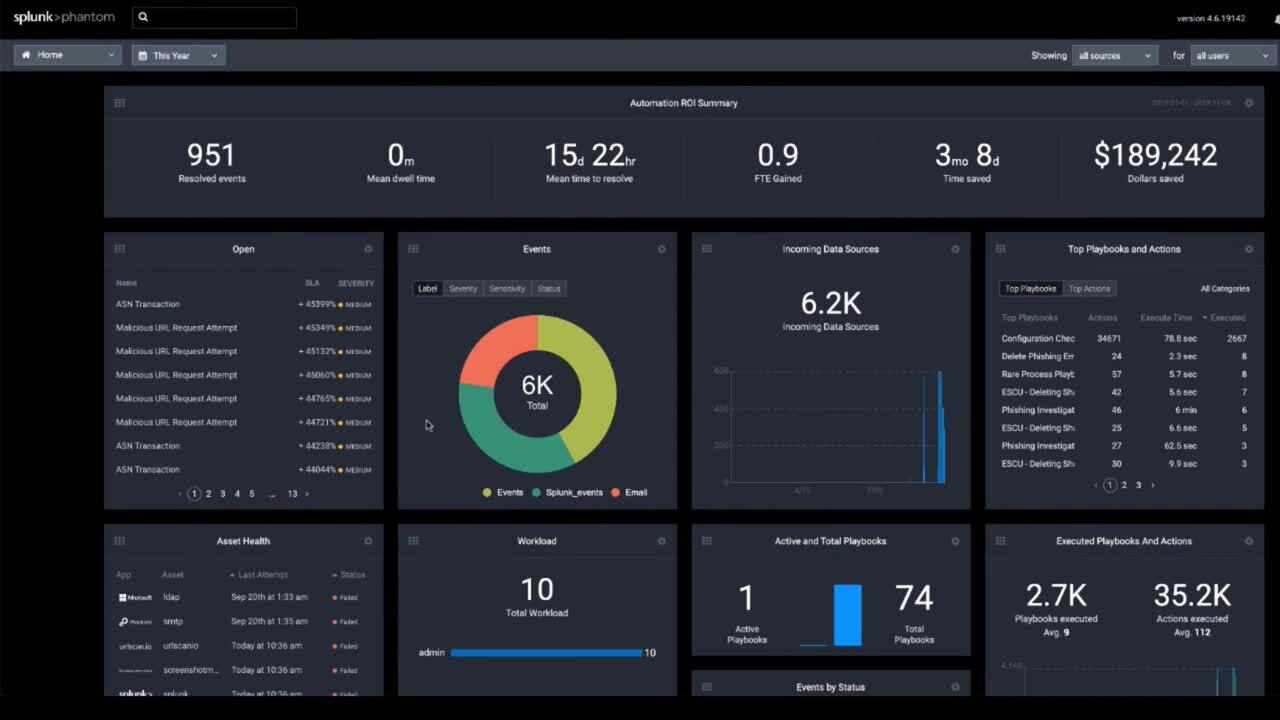
\includegraphics[width=0.9\textwidth]{images/splunk_soar_dashboard.jpg}
    \caption[Example of a Splunk SOAR dashboard]{Example of a Splunk SOAR dashboard. Such dashboards provide SOC teams with real-time visibility into security operations and response effectiveness.}
    \label{fig:splunk-soar-dashboard}
\end{figure}

In the implemented SOAR system, the dashboard consists of multiple interactive visual components:

\begin{itemize}
    \item \textbf{Pie Charts:} Used to represent incident distribution by severity (e.g., low, medium, high, critical) and status (e.g., open, in-progress, mitigated, closed).
    \item \textbf{Stacked Area Chart:} Visualizes the temporal trend of different incident categories, highlighting fluctuations and surges over time.
    \item \textbf{Bar Graph:} Displays the top attack types or event categories based on frequency, helping prioritize detection rules and playbook tuning.
    \item \textbf{Line Graph:} Shows overall incident volume over time, aiding in spotting recurring threat patterns or anomalies.
    \item \textbf{Mitigated Incidents Table:} Presents a detailed list of incidents that have been resolved, including timestamps, severity, method of mitigation, and analyst notes.
\end{itemize}

These visualizations are dynamically generated from the backend database, ensuring that the SOC team has access to up-to-date information. The use of modern front-end technologies allows filtering, hovering, and drill-down capabilities, enhancing usability for both Tier 1 analysts and SOC managers.

Comparatively, enterprise-grade SOAR platforms like \textbf{Splunk SOAR} and \textbf{Palo Alto Cortex XSOAR} also provide robust dashboard modules. Splunk SOAR’s dashboard includes customizable widgets that display automation coverage, playbook execution stats, case resolution times, and threat type breakdowns~\cite{splunk}. XSOAR offers executive summary views, threat intelligence overlays, SLA tracking, and integrations with MITRE ATT\&CK matrix visualizations~\cite{paloalto}. These features enable high-level stakeholders to monitor security posture, compliance adherence, and operational performance at scale.

Open-source platforms such as \textbf{Shuffle}, while more lightweight, offer basic dashboarding features focused on workflow execution success rates, recent runs, and task failures~\cite{techtarget}. Although minimal in comparison to commercial counterparts, Shuffle’s dashboard can be extended using third-party tools like Grafana or Kibana for deeper visibility.

Incorporating a rich dashboard module is essential for enabling data-driven incident response. It allows the SOC to not only track key performance indicators (KPIs) like Mean Time to Detect (MTTD) and Mean Time to Respond (MTTR), but also identify bottlenecks, repetitive alerts, or insufficient playbook coverage. A well-designed dashboard turns data into actionable insight, promoting operational maturity and continuous improvement.

\subsection{Incidents}

The \textbf{Incidents} module serves as the operational core of the SOAR platform, responsible for ingesting, displaying, and managing security alerts received from upstream systems such as Security Information and Event Management (SIEM) platforms. Once alerts are correlated and classified as actionable, they are stored in the incident management system, where analysts can interact with them through structured interfaces and automated workflows.

In the implemented SOAR system, incidents are displayed in an interactive, filterable table. Each row in the table represents an individual incident, enriched with metadata fields such as:

\begin{itemize}[noitemsep,topsep=0pt]
    \item \textbf{Timestamp:} The time at which the incident was triggered.
    \item \textbf{Attack Type:} Categorization based on the detected behavior (e.g., brute-force, phishing, malware).
    \item \textbf{Severity:} A rating (e.g., low, medium, high, critical) based on correlation rules or risk score.
    \item \textbf{Source and Destination IPs/Hosts:} Network context of the event.
    \item \textbf{Associated MITRE Technique IDs:} Tactic and technique labels for threat classification.
    \item \textbf{Status:} Indicates whether the incident is open, in progress, resolved, or closed.
\end{itemize}

Users can apply filters to view incidents by attack type, status, or severity, and initiate response actions directly from the interface. A key feature of this platform is the support for both \textbf{manual and AI-assisted incident status updates}. Analysts can choose to take manual action—such as marking an incident as mitigated—or they may delegate mitigation suggestions to a selected machine learning (ML) model, which recommends or executes responses based on historical resolution patterns.

\begin{figure}[ht]
    \centering
    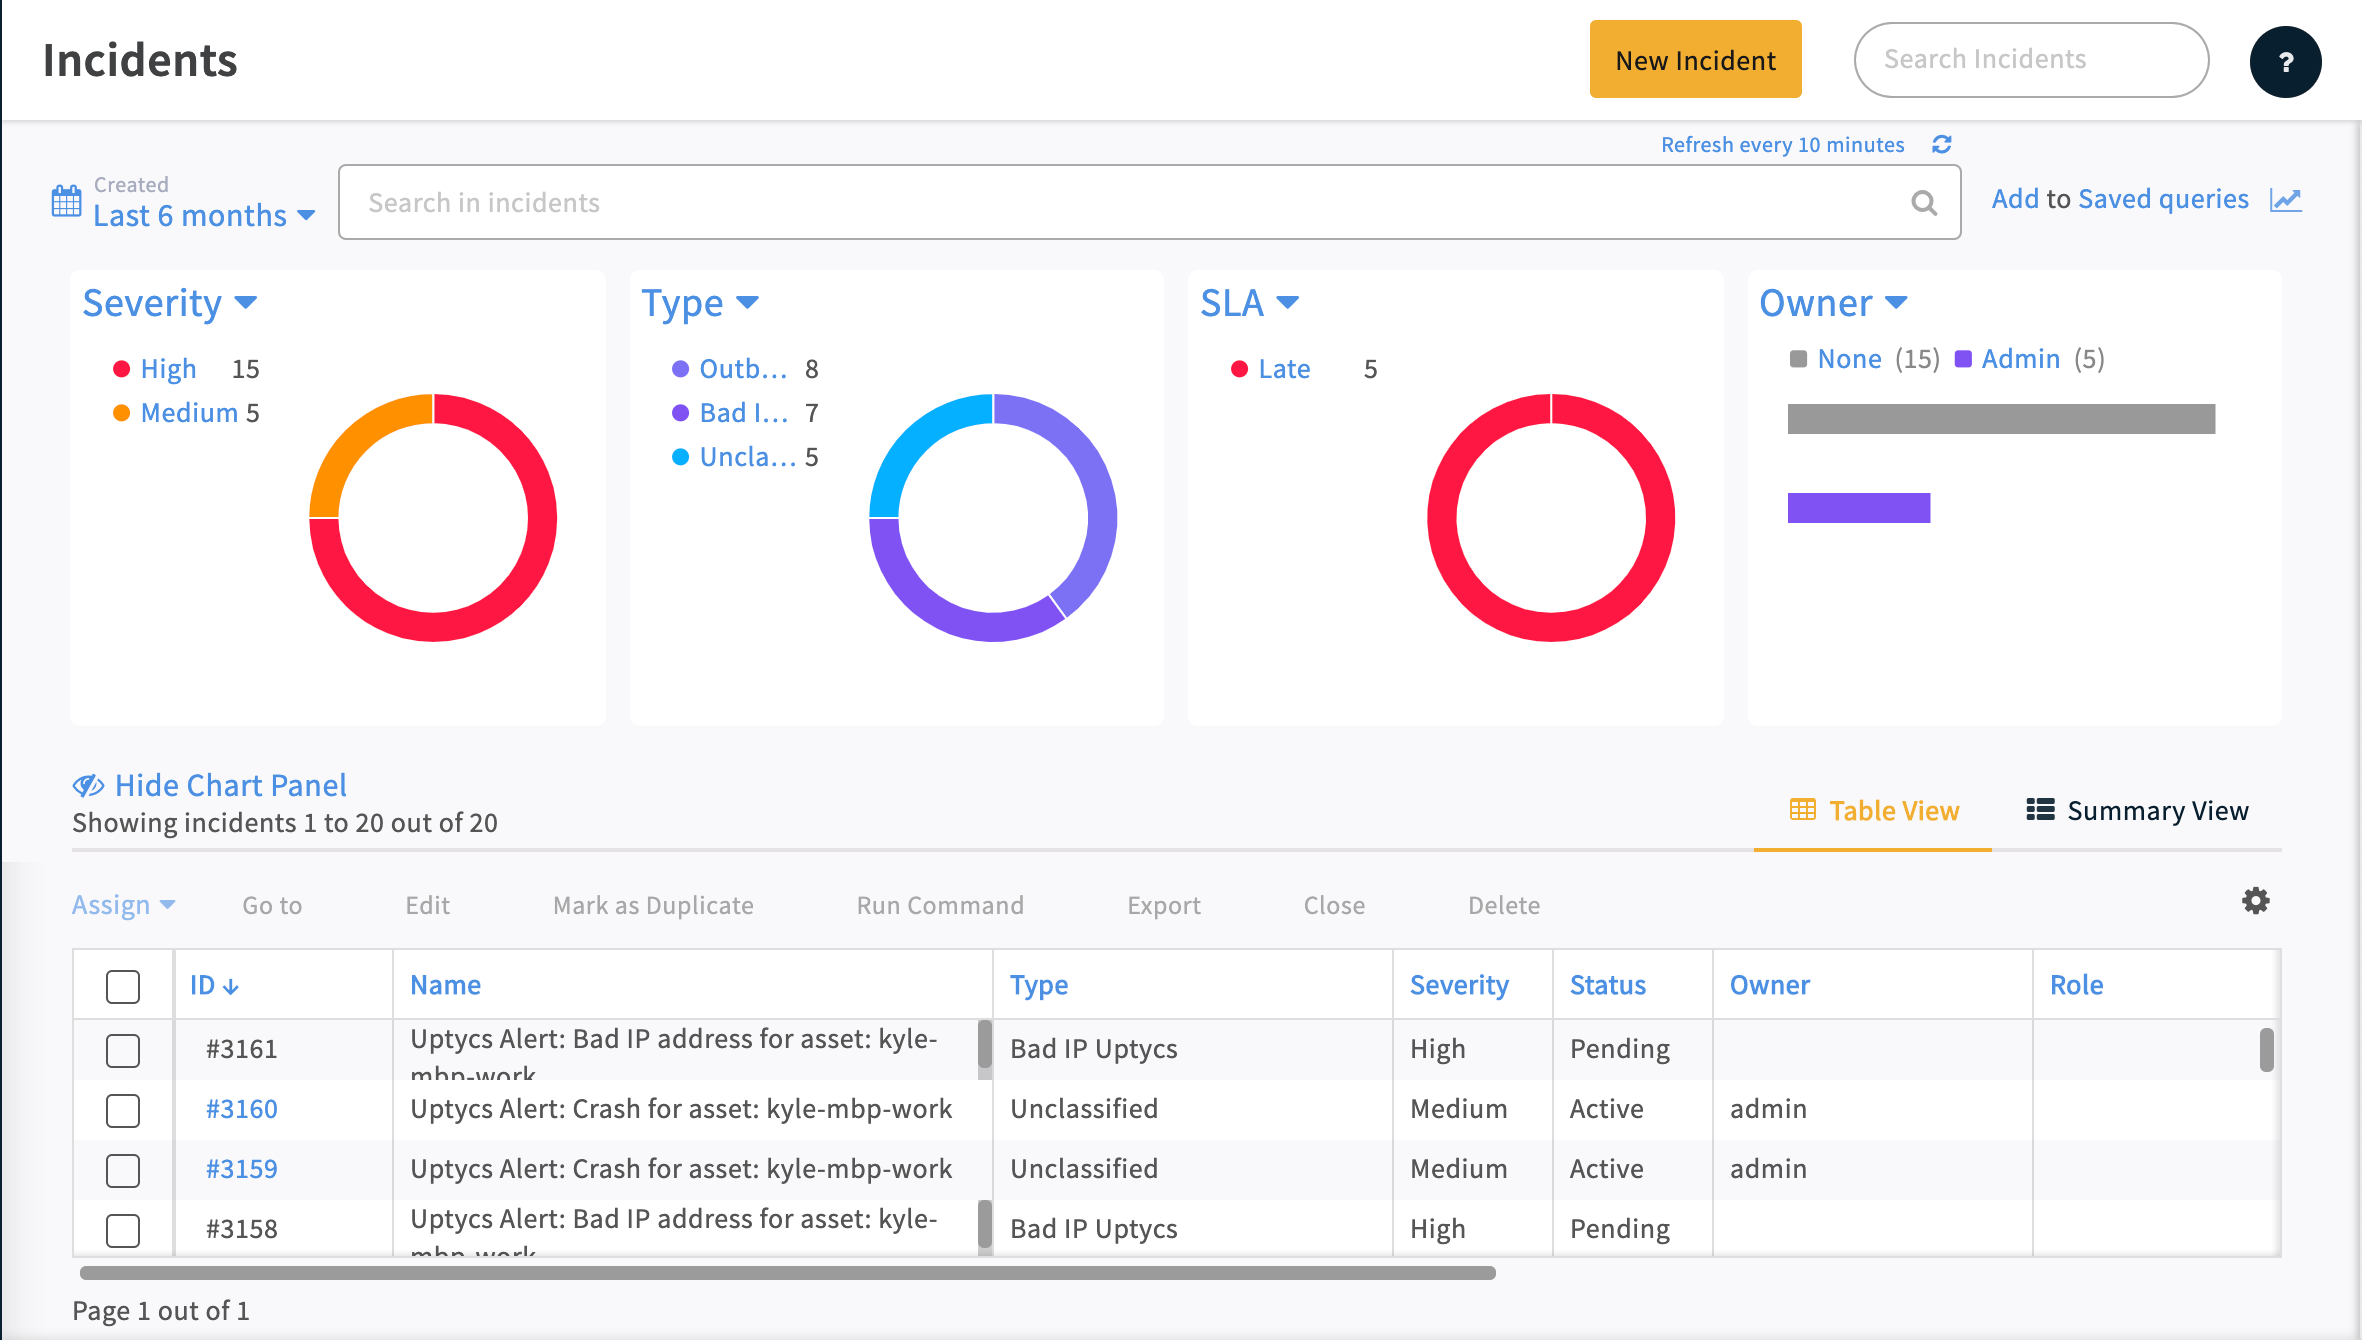
\includegraphics[width=0.9\textwidth]{images/xsoar_incidents.png}
    \caption[Incident management interface in Palo Alto Cortex XSOAR]{Incident management interface in Palo Alto Cortex XSOAR. The interface provides analysts with a comprehensive view of incidents, including filtering, status updates, and detailed metadata for each alert.}
    \label{fig:xsoar-incidents}
\end{figure}

This AI-based mitigation capability is a significant enhancement over many commercial SOAR platforms, where AI and ML integration is either minimal or handled externally. For example, while \textbf{Splunk SOAR} provides advanced correlation and playbook automation, it does not natively include ML model selection or self-learning response recommendation without integration with third-party platforms~\cite{splunk}. Similarly, \textbf{Cortex XSOAR} enables data enrichment and contextual awareness, but machine learning functionalities often rely on Palo Alto’s Threat Intelligence or external sources~\cite{paloalto}.

Open-source SOAR tools like \textbf{Shuffle} provide basic incident ingestion and display via webhook integrations, but lack built-in enrichment, severity scoring, or AI-assisted resolution workflows~\cite{techtarget}. The presented SOAR system thus bridges this gap by offering native ML model selection for predictive mitigation, making it suitable for organizations that want to experiment with or deploy AI-driven security automation.

In addition, the incident module supports direct association with MITRE ATT\&CK techniques, enabling targeted response and heatmap generation. When combined with the playbook engine, this allows the automatic execution of workflows based on specific tactics or techniques observed in the incident.

In conclusion, the incident module in the custom SOAR platform not only visualizes threat data but actively integrates with intelligence, analytics, and automation components. Its hybrid approach—combining analyst control with AI support—ensures scalability, consistency, and reduced mean time to respond (MTTR) in SOC operations.

\subsection{Integrations}

The \textbf{Integrations} module is a foundational component of any SOAR platform, enabling connectivity and orchestration across a diverse ecosystem of cybersecurity tools and services. It allows the platform to interact with third-party systems—such as firewalls, endpoint protection platforms (EPP/EDR), threat intelligence feeds, vulnerability scanners, cloud providers, and ticketing systems—through standardized API-based interfaces. This connectivity is essential to execute automated actions during playbook execution or manual analyst workflows.

In the implemented SOAR platform, integrations are managed via a dedicated interface that allows the creation, modification, and deletion of both \textbf{Apps} and their corresponding \textbf{Actions}:

\begin{itemize}
    \item \textbf{App:} Represents an external service or tool. Each app includes fields such as \textit{name}, \textit{description}, and \textit{API token} or other required authentication information.
    \item \textbf{Action:} Represents a specific operation that the app can perform. Each action includes an \textit{action\_name}, the \textit{HTTP method} (GET, POST, PUT, DELETE), and the \textit{API endpoint URL}.
\end{itemize}

These definitions allow non-technical users to register integrations and reuse them across multiple workflows without writing code. Once configured, the actions can be triggered from playbooks or manually executed from the incident module. For example, a configured VirusTotal app might have actions like `scan\_url`, `check\_hash`, or `get\_report`, which can be called during threat enrichment.

Compared to commercial solutions, this modular app-action model is aligned with industry best practices. \textbf{Splunk SOAR}, for instance, provides over 300 built-in integrations known as “apps,” each containing a set of pre-configured actions. These can be used in visual playbooks and extended via custom Python scripting~\cite{splunk}. Similarly, \textbf{Cortex XSOAR} organizes integrations into packs that include playbook tasks, data models, and API-based connectors~\cite{paloalto}. It also supports live configuration from the user interface and centralized credential management.

Open-source platforms such as \textbf{Shuffle} follow a comparable model by offering REST-based integrations that can be created or imported from community repositories. Shuffle also allows users to write lightweight custom apps in Python or JavaScript, which are run in sandboxed Docker containers~\cite{techtarget}.

\begin{figure}[ht]
    \centering
    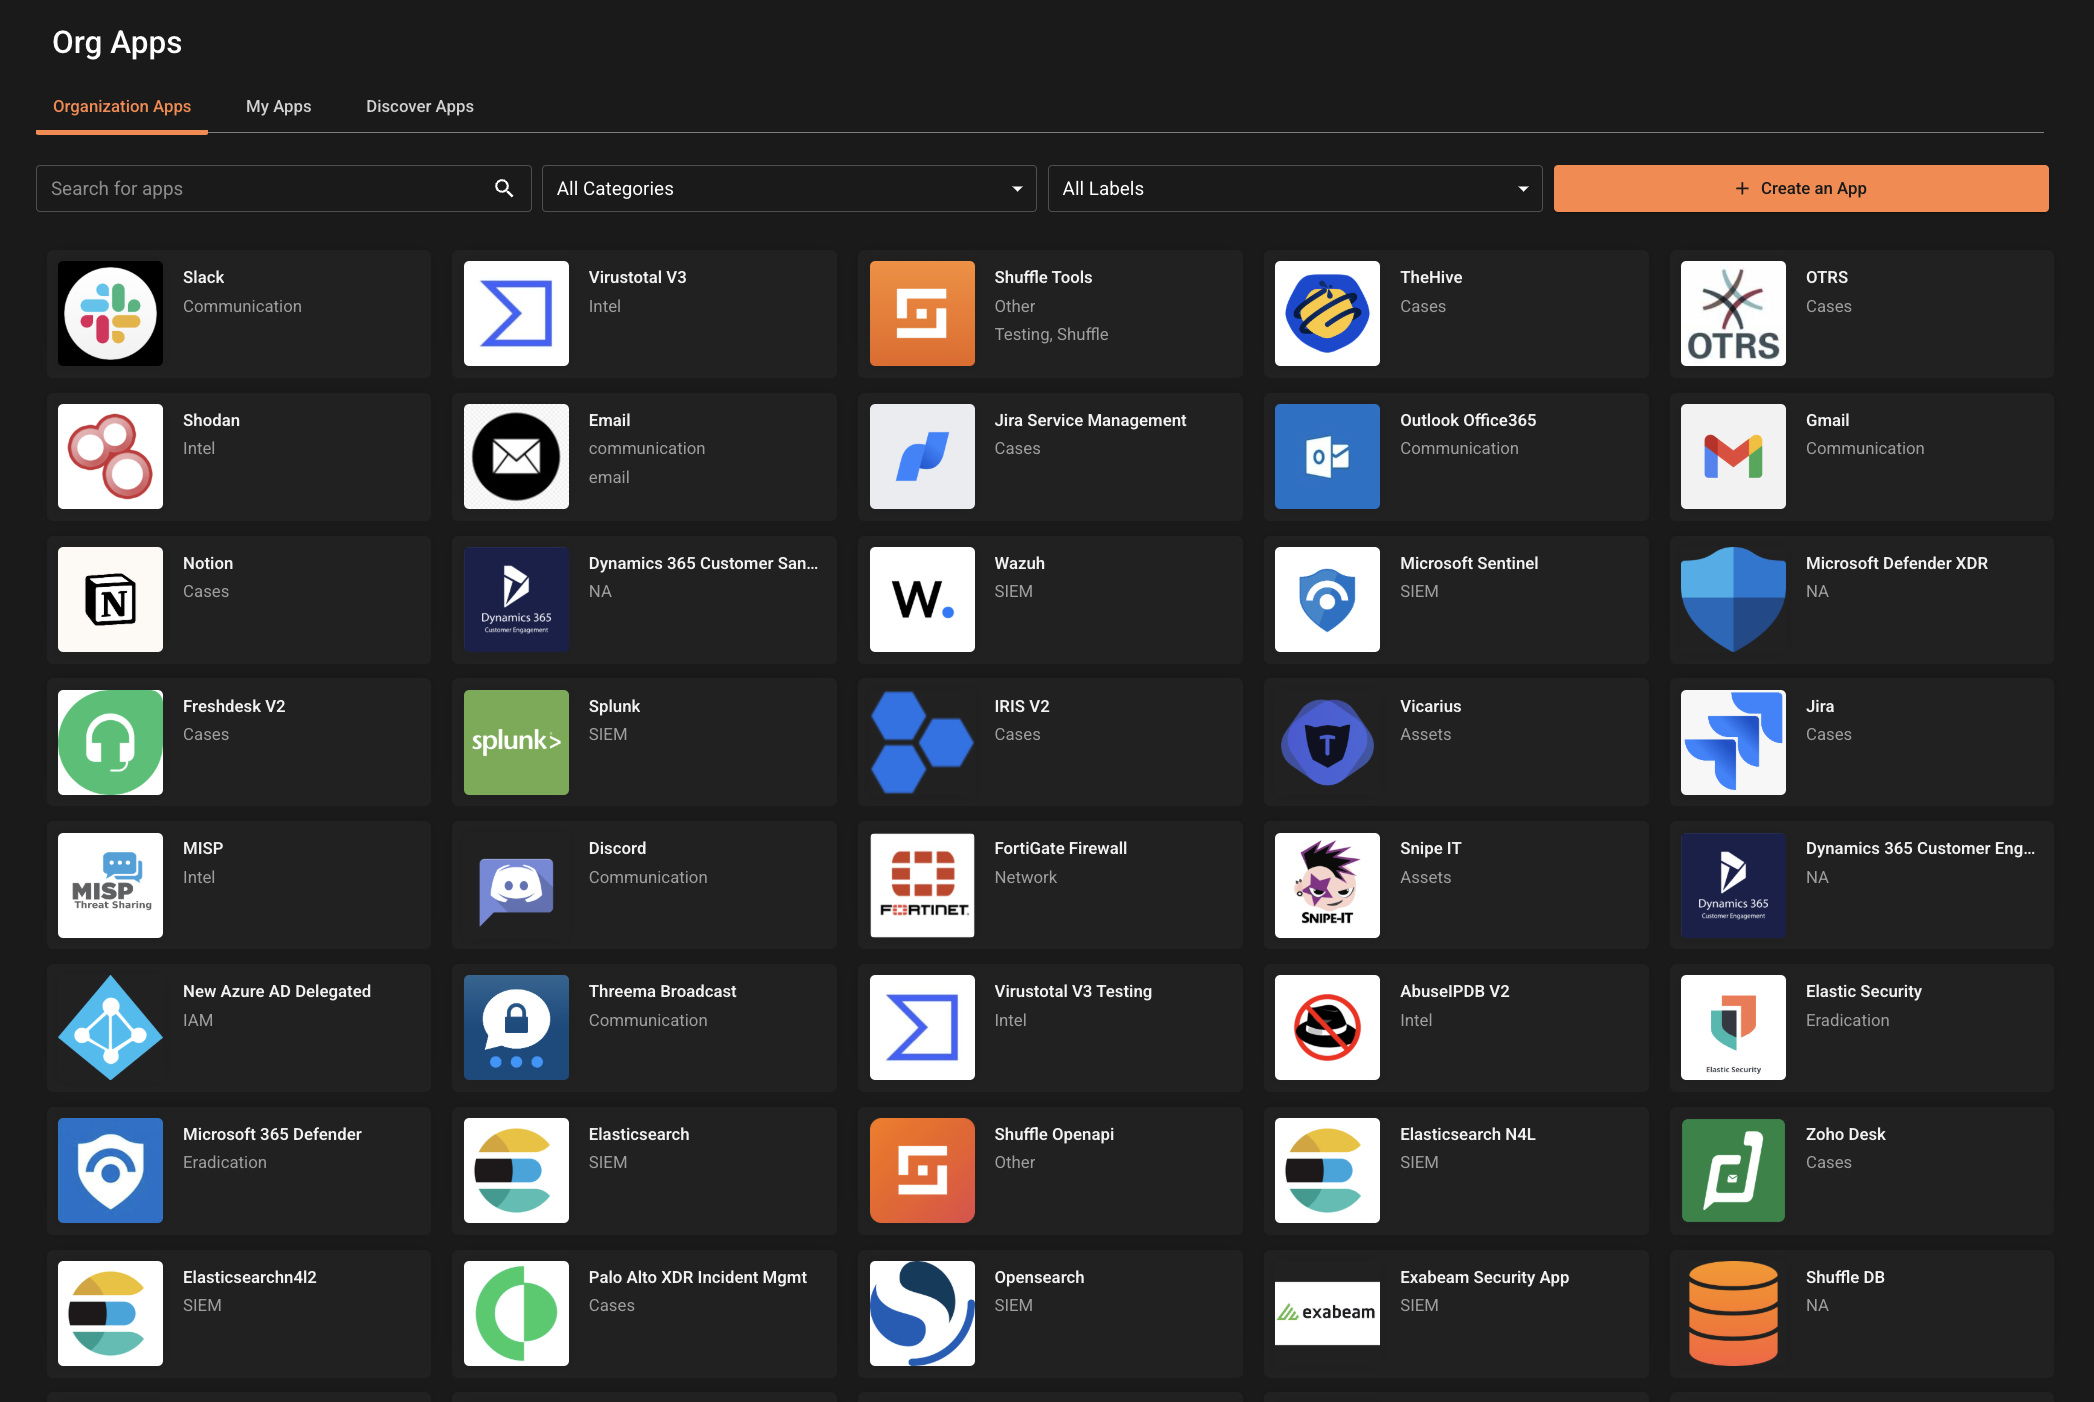
\includegraphics[width=0.9\textwidth]{images/shuffle_soar_apps.png}
    \caption[[Example of the integrations (apps) interface in Shuffle SOAR]]{Example of the integrations (apps) interface in Shuffle SOAR. Users can visually manage and configure third-party integrations and their actions through a web-based UI.}
    \label{fig:shuffle-soar-apps}
\end{figure}

One of the distinguishing features of the custom SOAR platform developed during this internship is the ability to define integrations dynamically through the web interface, without requiring backend changes or container redeployments. This approach supports rapid integration with custom in-house tools, threat intelligence APIs, or security appliances used in air-gapped and defense environments. Since each integration is abstracted into reusable action objects, users can visually link them into workflows using the workflow builder module.

The integrations module not only enhances automation but also ensures scalability and modularity in security operations. By treating each external service as a pluggable app with configurable actions, the platform adheres to microservice principles, making it extensible for future orchestration needs.

\subsection{Playbooks}

The \textbf{Playbooks} module is the automation engine of the SOAR platform, enabling structured and repeatable responses to detected security incidents. A playbook is a predefined sequence of steps—both automated and manual—that governs how an incident should be investigated and remediated. Playbooks are essential for ensuring consistency, reducing analyst fatigue, and minimizing human error in high-volume environments.

In the implemented SOAR system, playbooks are defined, managed, and executed via an intuitive user interface. The module supports the following key features:

\begin{itemize}[noitemsep,topsep=0pt]
    \item \textbf{Add/Edit/Delete Playbook:} Users can create new playbooks or modify existing ones to align with updated procedures, threat types, or compliance requirements.
    
    \item \textbf{MITRE ATT\&CK Association:} Each playbook can be linked to one or more MITRE ATT\&CK Technique IDs. When an incoming incident matches a technique identifier, the corresponding playbook is automatically triggered. This enables context-aware, tactic-specific response automation~\cite{mitre}.
    
    \item \textbf{Workflow Linking:} Playbooks are tied to workflows—graphical representations of the actions and conditions to be executed in sequence. This decouples the logical decision-making layer (playbooks) from the execution engine (workflow), promoting reuse and flexibility.
\end{itemize}

The logic defined within a playbook may include various response actions, such as:
\begin{itemize}[noitemsep,topsep=0pt]
    \item Enriching indicators using threat intelligence sources (e.g., WHOIS, VirusTotal).
    \item Blocking malicious IPs or URLs using integrations with firewalls or web gateways.
    \item Isolating endpoints using EDR tools.
    \item Creating tickets or notifications via ticketing systems or email services.
\end{itemize}

Each step can include conditions, triggers, and optional human approvals, allowing playbooks to function in fully automated or semi-automated modes.

This implementation follows the design philosophy of enterprise-grade SOAR platforms. For instance, \textbf{Splunk SOAR} allows users to build playbooks using a visual editor, combining decision blocks, automation tasks, and manual inputs~\cite{splunk}. Playbooks in Splunk SOAR are Python-based under the hood but are abstracted for low-code use. \textbf{Palo Alto Cortex XSOAR} extends this concept with its drag-and-drop playbook editor and built-in task types, enabling advanced branching logic and error handling~\cite{paloalto}.

Open-source SOAR platforms such as \textbf{Shuffle} also provide playbook editors with visual flow-based design. However, they are typically limited in features such as conditional branching, versioning, and advanced user inputs~\cite{techtarget}. While sufficient for basic automation, they may require custom scripting for more complex response procedures.

A unique aspect of the custom SOAR platform presented in this work is its ability to associate playbooks with ATT\&CK techniques directly within the interface, thereby enabling seamless tactic-level incident automation. This facilitates faster and more accurate responses, especially in SOC environments aligned with the MITRE ATT\&CK framework for threat modeling and incident classification.

Overall, the playbook module is instrumental in operationalizing security response strategies. It encapsulates institutional knowledge, codifies best practices, and ensures that each incident is handled with appropriate urgency and consistency.

\subsection{Workflows}

The \textbf{Workflow} module acts as the execution engine of the SOAR platform, responsible for carrying out the actions defined within playbooks. While playbooks provide the logical structure and decision-making rules for incident response, workflows are the operational blueprints that determine how tasks are executed in sequence—visually represented as directed graphs composed of nodes (apps/actions) and edges (transitions).

In the developed SOAR platform, workflows are created and managed using a visual, drag-and-drop interface. Key features of the module include:

\begin{itemize}
    \item \textbf{Create/Edit/Delete Workflows:} Users can construct workflows from scratch or modify existing ones using a canvas-based editor.
    
    \item \textbf{Node-Based Design:} Each node represents an app configured via the Integrations module. Nodes may expose one or more actions (e.g., scan file, block IP, query URL).
    
    \item \textbf{Drawable Edges:} Nodes are connected using directional edges to define the order of execution. Conditional routing and branching logic can be visually represented by linking multiple nodes based on success, failure, or other states.
    
    \item \textbf{Execution List:} A log of previously executed workflows is maintained, including execution status, incident ID, trigger source, timestamps, and logs for each step.
\end{itemize}

This approach provides SOC analysts with a low-code environment to model complex incident response logic visually, making it accessible to both technical and non-technical users. Analysts can reuse workflows across different playbooks, promoting modularity and standardization in the response process.

The architecture of the workflow module is conceptually similar to what is offered by commercial SOAR platforms. For example, \textbf{Splunk SOAR} includes a visual playbook editor where each block represents a discrete action or condition, forming a directed flowchart~\cite{splunk}. Actions can be executed in sequence or in parallel, with support for user prompts, decision gates, and failure handling.

\begin{figure}[ht]
    \centering
    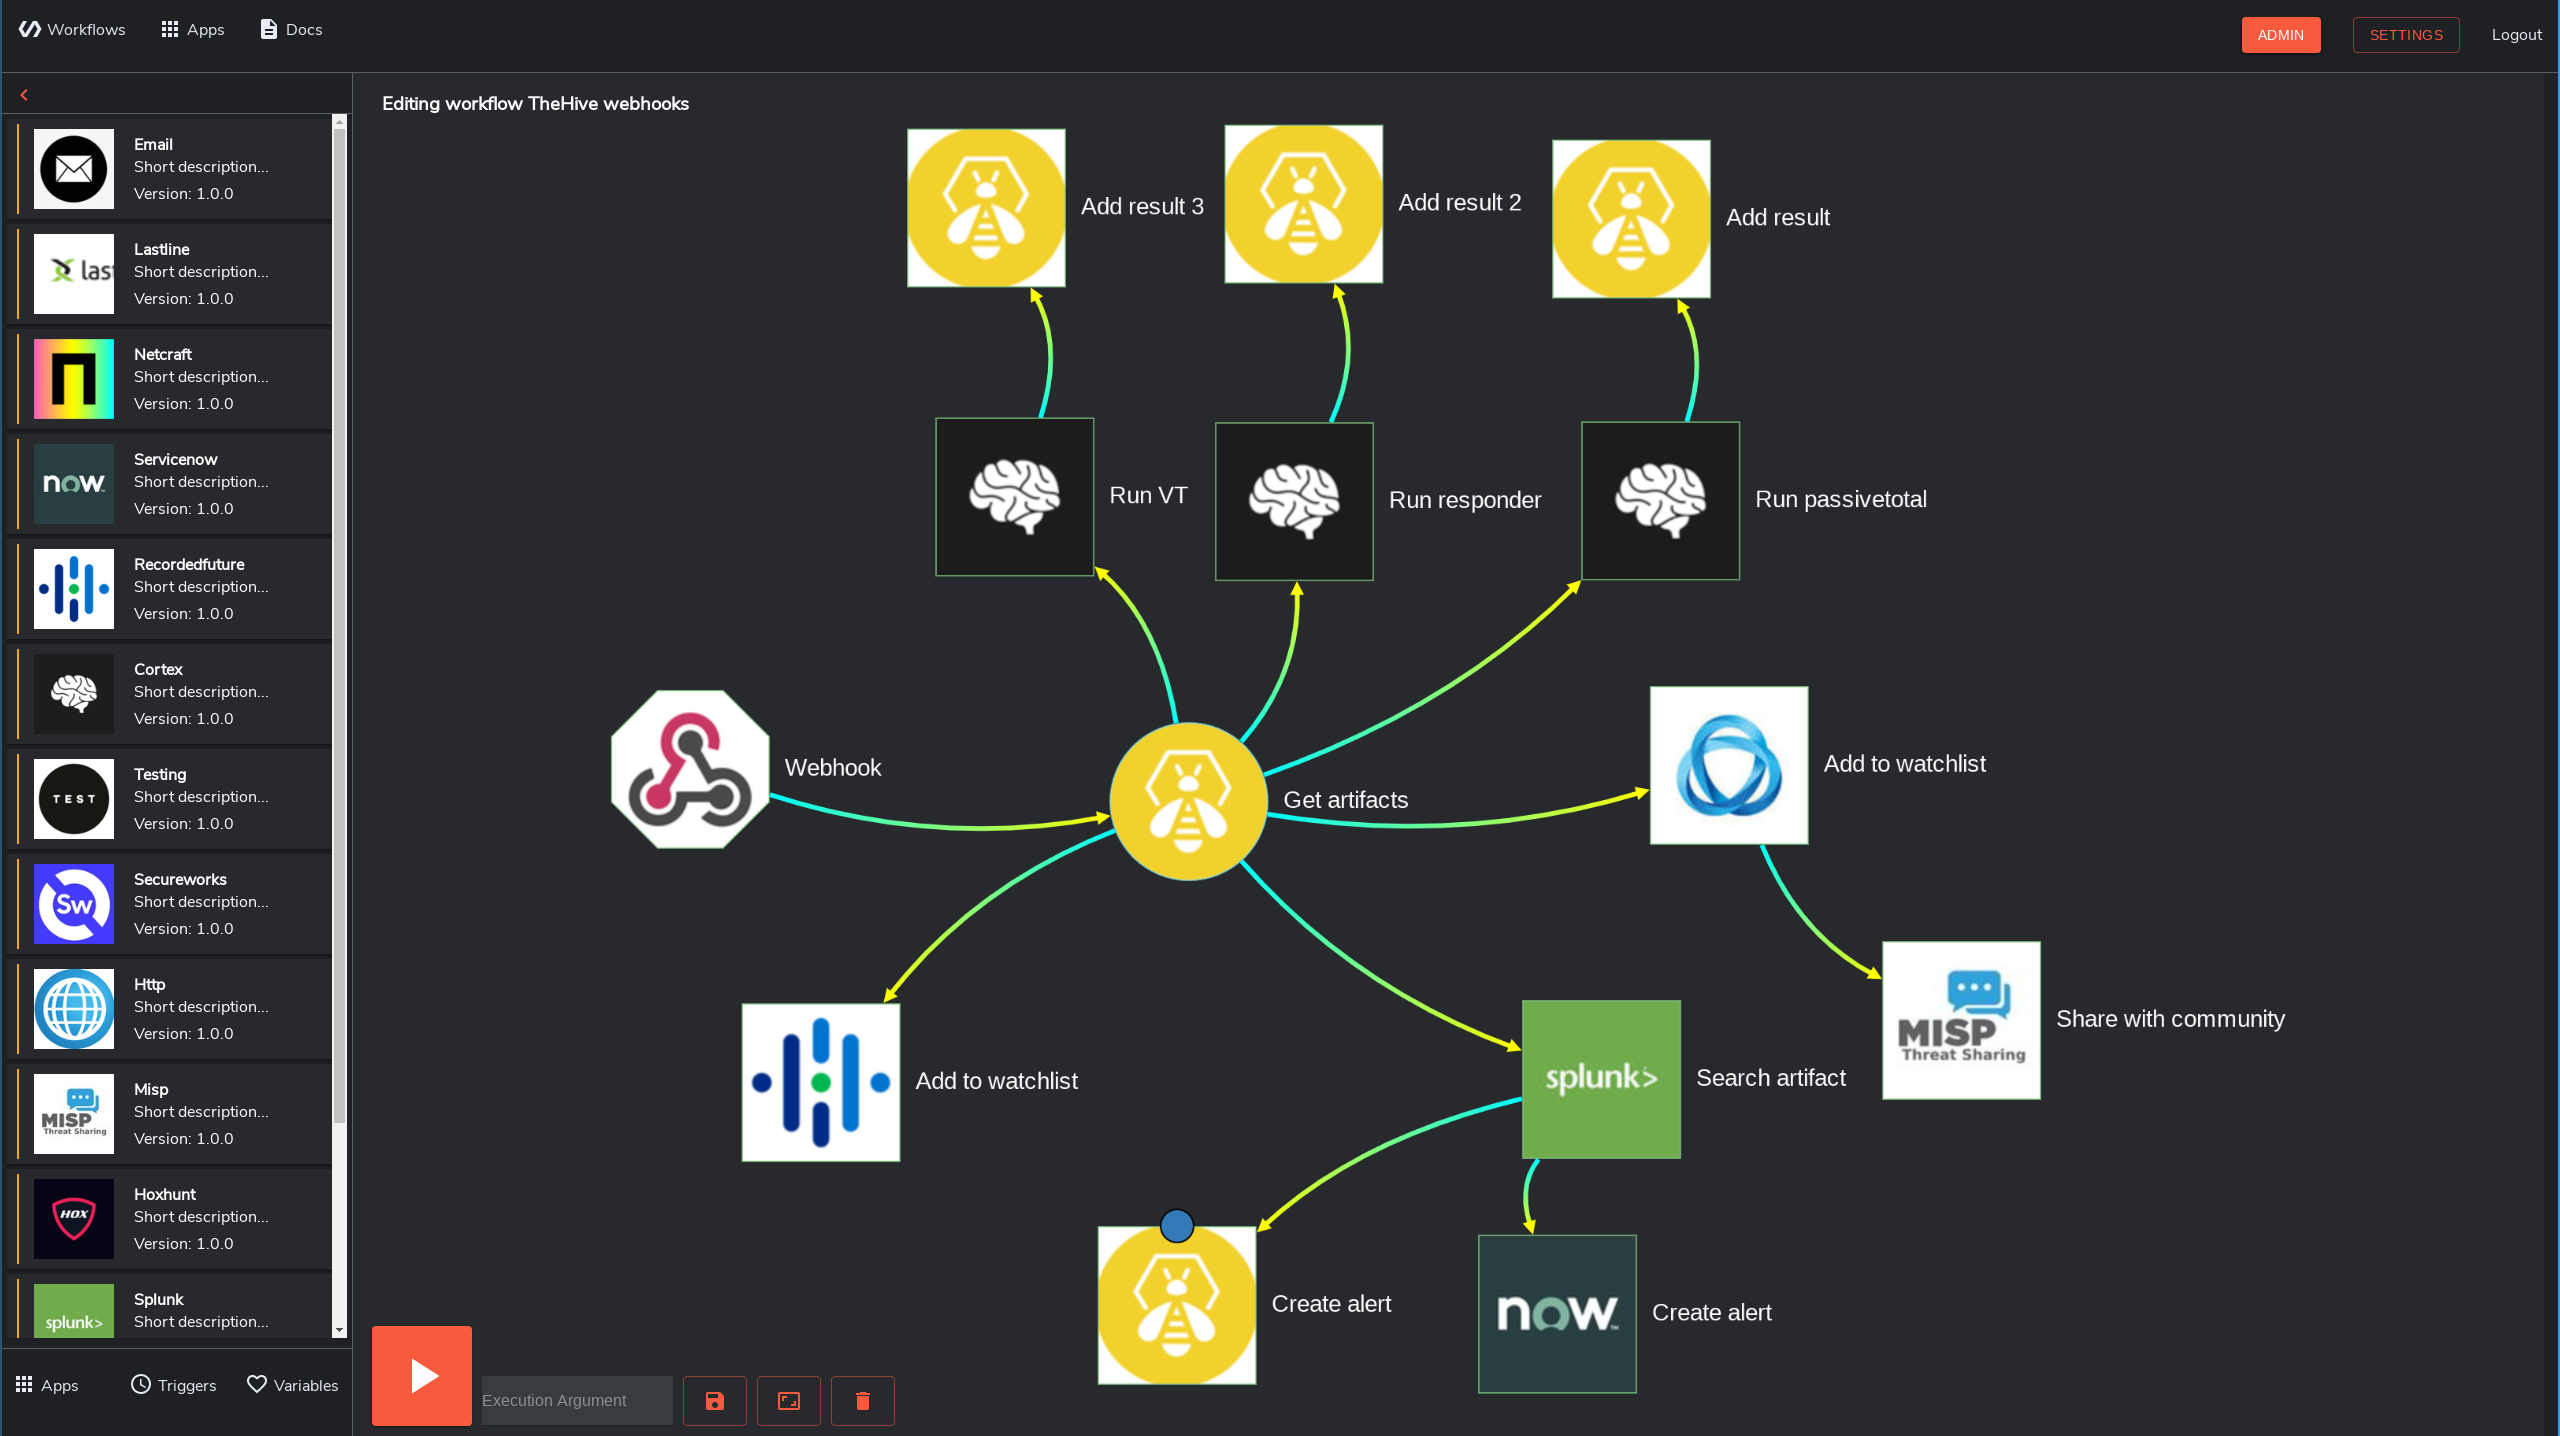
\includegraphics[width=0.9\textwidth]{images/shuffle_soar_workflow.png}
        \caption[Example of a workflow editor in Shuffle SOAR]{Example of a workflow editor in Shuffle SOAR. The visual interface allows users to design and manage automated response workflows by connecting integration actions and defining execution logic.}
    \label{fig:shuffle-soar-workflow}
\end{figure}

\textbf{Palo Alto Cortex XSOAR} extends this paradigm by offering sophisticated conditional flows, loops, exception management, and variable sharing across tasks~\cite{paloalto}. Its workflow engine supports both automation tasks and human-in-the-loop interactions (e.g., approval requests), enabling hybrid response models.

Open-source SOAR platforms such as \textbf{Shuffle} are also designed around workflow automation, with a visual interface that allows drag-and-drop placement of integration actions, conditional paths, and data variables~\cite{techtarget}. However, Shuffle workflows typically focus on simplicity and ease of scripting, with fewer built-in safeguards or error-handling mechanisms compared to enterprise-grade systems.

A distinctive aspect of the workflow module in the custom SOAR platform is its tight coupling with the Integrations and Playbook modules. Users can dynamically select app actions while building workflows, and these workflows can be associated with specific playbooks tied to MITRE ATT\&CK techniques. This modularity allows for flexible reuse, rapid prototyping, and seamless expansion as new integrations and response use cases are added.

Overall, the workflow module transforms logical response strategies into executable sequences, providing the backbone for effective security automation in the SOAR architecture. It bridges the gap between decision logic and operational execution, ensuring that incident handling is both efficient and auditable.

\subsection{MITRE ATT\&CK Module}

The \textbf{MITRE ATT\&CK} (Adversarial Tactics, Techniques, and Common Knowledge) module integrates the widely adopted threat modeling framework into the SOAR platform to enhance contextual awareness, incident classification, and strategic response alignment. ATT\&CK provides a structured knowledge base of adversary behaviors, organized into tactics (goals) and techniques (methods), allowing SOC teams to understand the “why” and “how” behind detected threats~\cite{mitre}.

In the developed SOAR system, the MITRE ATT\&CK module offers a visually interactive matrix interface modeled after the official ATT\&CK Enterprise Matrix. Its key features include:

\begin{itemize}
    \item \textbf{Technique-Based Filtering:} Each cell in the matrix corresponds to a specific ATT\&CK technique. Clicking on a cell filters and displays the list of incidents in the system that are mapped to that technique, providing quick threat attribution.
    
    \item \textbf{Heatmap Visualization:} A color-coded heatmap overlays the matrix based on the number of incidents associated with each technique. Colors range from white (no incidents) to blue (low frequency) to red (high frequency), visually highlighting the most frequently observed techniques within the environment.
    
    \item \textbf{Technique-Incident Association:} During incident ingestion, techniques can be mapped automatically or manually, linking each incident to its corresponding ATT\&CK entries. This classification is leveraged by playbooks to determine which workflows to trigger.
\end{itemize}

The integration of MITRE ATT\&CK in SOAR platforms serves multiple purposes: it enhances situational awareness, supports threat hunting, and allows for better alignment of detection and response strategies with real-world adversary tactics. Furthermore, it provides a foundation for behavioral analytics, red teaming, and compliance reporting.

Commercial SOAR solutions such as \textbf{Palo Alto Cortex XSOAR} offer built-in support for ATT\&CK. Incidents can be tagged with tactics and techniques, and dashboard modules allow visualization of coverage and attack surface exposure~\cite{paloalto}. XSOAR also supports threat intel enrichment using ATT\&CK metadata and enables filtering and reporting based on technique distributions.

\textbf{Splunk SOAR} does not natively provide a full ATT\&CK matrix interface, but integrations with the Splunk Security Essentials app or external visualizations (e.g., MITRE ATT\&CK Navigator) allow SOCs to map playbooks and detections to tactics and techniques~\cite{splunk}.

\begin{figure}[ht]
    \centering
    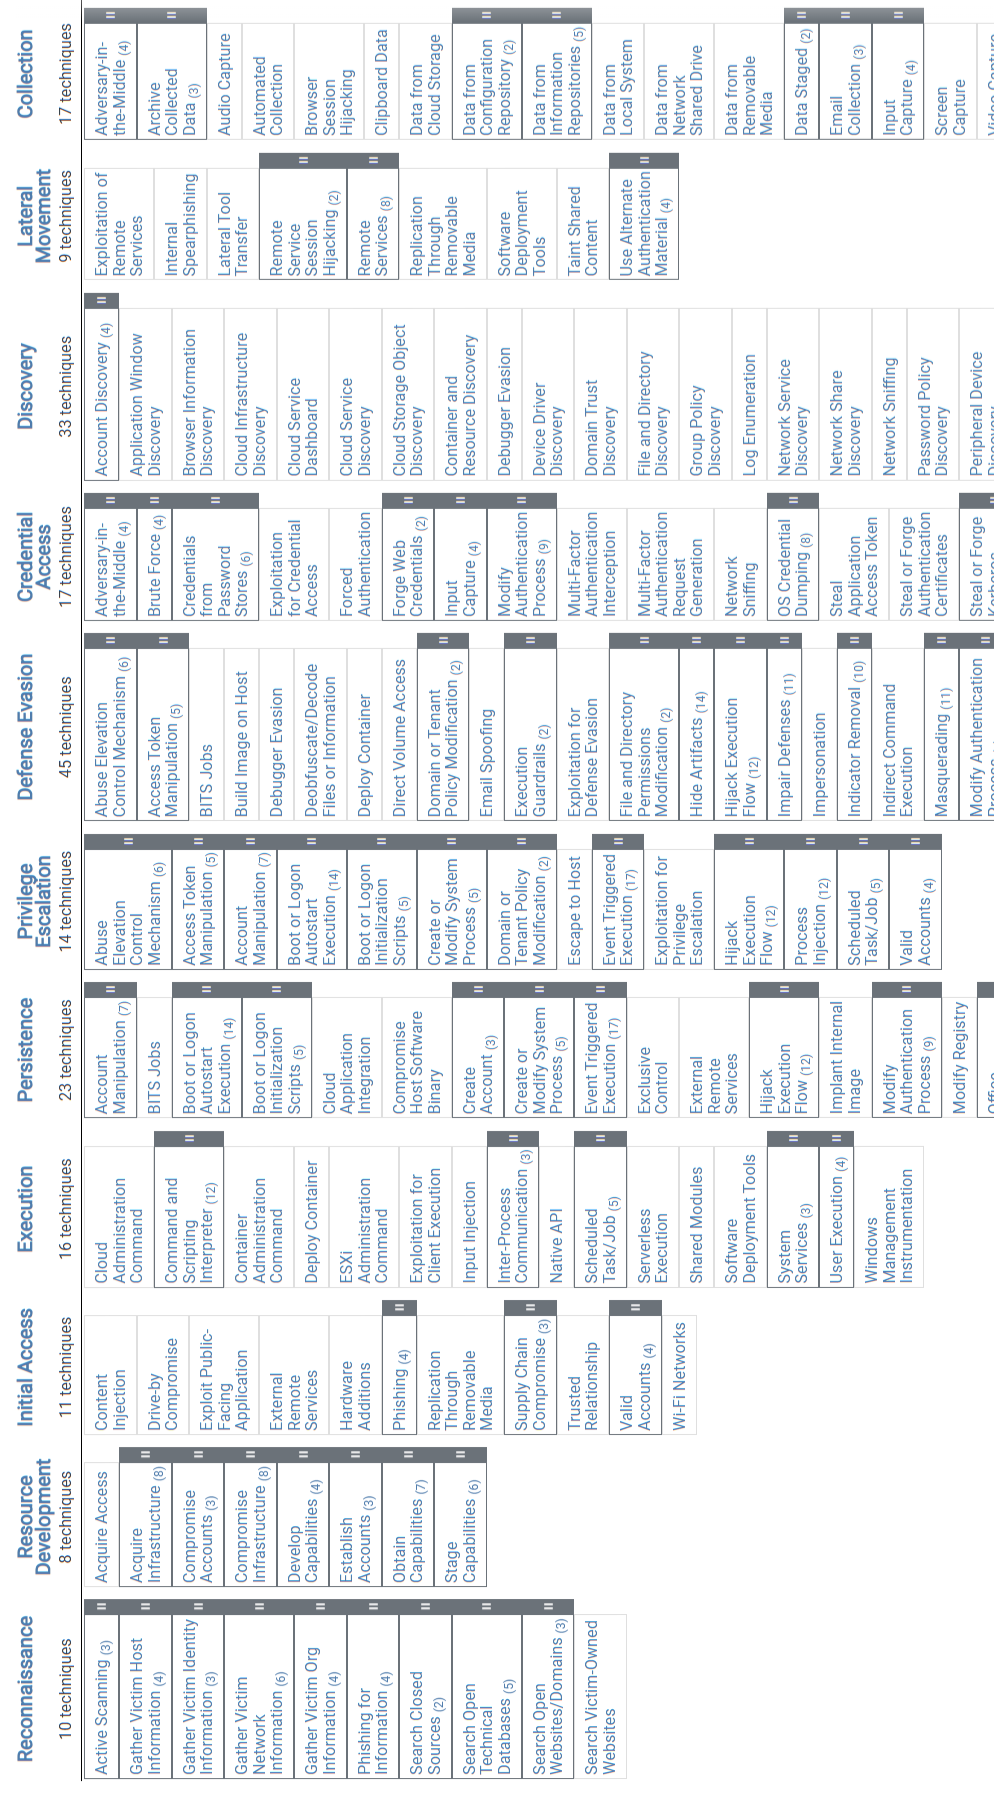
\includegraphics[width=0.9\textwidth]{images/mitre_att&ck_matrix.png}
    \caption[Interactive MITRE ATT\&CK matrix]{Interactive MITRE ATT\&CK matrix. The matrix enables analysts to visualize incident distribution across tactics and techniques, supporting rapid threat attribution and response prioritization.}
    \label{fig:mitre-attck-matrix}
\end{figure}

Open-source platforms such as \textbf{Shuffle} generally do not include a dedicated ATT\&CK interface out-of-the-box, though users can manually tag incidents and build custom visualizations using third-party tools like ATT\&CK Navigator, Kibana, or D3.js-based dashboards~\cite{techtarget}.

The custom SOAR platform presented here integrates ATT\&CK directly into its core, offering a native visual matrix tightly coupled with incident metadata and playbook execution. By embedding this visualization, analysts gain immediate insight into threat patterns and can prioritize response actions based on frequently exploited techniques. This also supports proactive defense strategies, such as identifying unmonitored or under-covered techniques and adapting detection rules accordingly.

Overall, the MITRE ATT\&CK module elevates the strategic value of the SOAR platform, enabling structured threat intelligence application, better prioritization, and improved operational alignment with adversary behaviors.